\setlength\intextsep{1mm}

\section*{\textbf{Task 1: Classification of diabetes with K-fold cross-validation}}

\textbf{1.} Report on choices of \textbf{K fold}, \textbf{normalization method}, \textbf{Cost function}.

\begin{table}[H]
    \centering
    \begin{tabular}{|c|c|}
    \hline
         Model details &  Choice  \\
        \hline
         K fold & 4 \\
         Normalization method & standard normalization   \\
         Cost function & two-class softmax cost function   \\
        \hline
    \end{tabular}
    \caption{Choices for tuning the linear two-class classification problem}
    \label{tab:model choices}
\end{table}

\textbf{Reasoning: }
\begin{itemize}
    \item K=4 fold was used. This was due to the limited data point (total=72) we have. At the beginning, we also need to split 20\% (15 data points) out as the testing data. With such limited data point for traing and cross-validation (57 data points), the cross-validation splits should use more data for training so as to capture the underlying phenomenon.
    \item training data was pre-processed using standard normalization. This method just centers and standardizes the dataset. The final trained weight attached to each feature dimension is preserved such that the final model is easier to inteprete the importance of features. (However, if PCA sphering is used, the importance of features might not be this direct since each principle is a mixture from all features.)
    \item The two-class softmax cost function with the \textbf{l1 norm} regularizer added is used.
    \begin{align*}
        g(w) = \frac{1}{P} * ( \sum_{p=1}^{P} log (1+e^{(-y_p * \dot{x}_p^T *w)}) + \lambda * \sum_{i}  | \textbf{w}_{feature_touching}^i | )
    \end{align*} 
\end{itemize}

\textbf{2.} Hyperparameter searching and the final choice.

To search for the suitable hyperparameters (learning rate $\alpha$ and regularizer factor $\lambda$), I adopted a grid searching procedure shown as the following table:


\begin{table}[H]
    \centering
    \begin{tabular}{c|ccccc}
    $\lambda$ \textbackslash $\alpha$ & 
    0.1000  &  0.0500  &  0.0100  &  0.0010  &  0.0001 \\
    \hline
        5 &    1.0 & 0.321429 & \textcolor{red}{\textbf{0.035714}} & 0.071429 & 0.142857 \\
        2 &   1.0   &   0.75 & 0.053571 & 0.107143 & 0.214286 \\
        1 &   1.0 & 0.517857 & 0.053571   &  0.125 & 0.285714 \\
        0.100  &  1.0 & 0.553571  &   0.125 & 0.267857 & 0.357143 \\
        0.050  &  1.0  &   0.625 & 0.214286 & 0.267857   &  0.375 \\
        0.010  &  1.0 & 0.660714 & 0.267857 & 0.303571   &  0.375 \\ 
        0.001  &  1.0 & 0.660714 & 0.285714 & 0.321429  &   0.375 \\
        \hline
    \end{tabular}
    \caption{Averaged validation error for combinations of $\alpha$ and $\lambda$}
    \label{tab:Averaged validation error}
\end{table}

\textbf{As highlighted in the table (bold \& red text), when using a $\alpha$ = 0.01 and a $\lambda$ of 5, the validation error reaches the lowest (0.0357), meaning that we can achiveve 96.43\% accuracy on average during cross-validation.}



\textbf{3.} Plot of cost vs. iteration of my final model over the entire training set.


\begin{figure}[H]
    \centering
    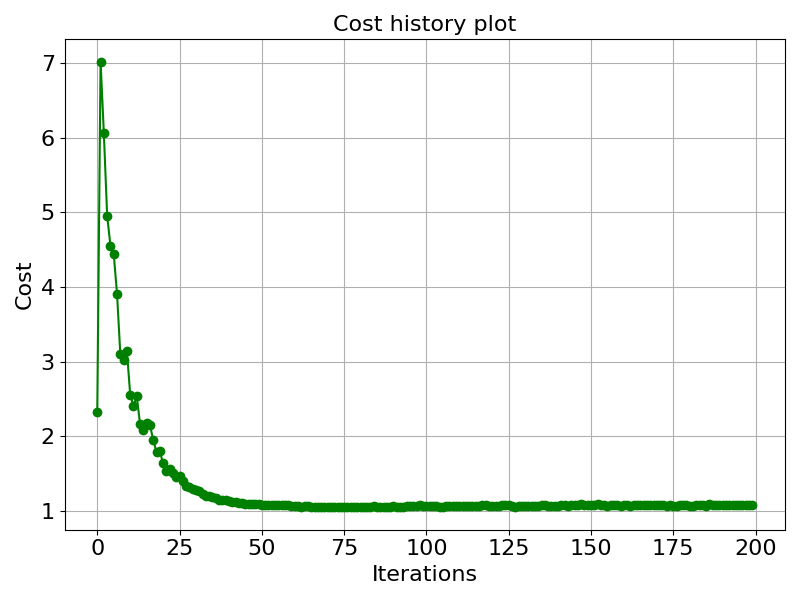
\includegraphics[width=120mm]{Cost_history_on_training_set.png}
    \caption{Cost history plots over 200 iterations}
    \label{fig:cost history}
\end{figure}


\textbf{Accuracy of my final model on the testing set: 100\%}

\textbf{4.} The 5 most influential genes in descending order.

\begin{figure}[H]
    \centering
    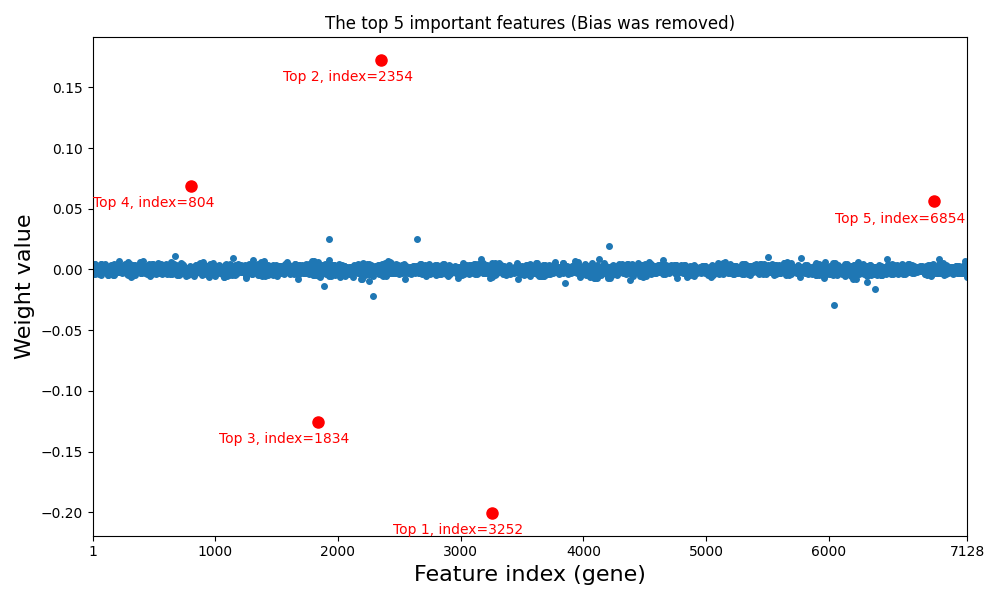
\includegraphics[width=160mm]{top-5-important features.png}
    \caption{The 5 most important feaures}
    \label{fig:Feature-touching weights}
\end{figure}

\textbf{As shown by Figure 2, the top 5 important features are 3252, 2354, 1834, 804, 6854. (after taking away the bias, the index shown in the figure starts from index 1, which is the first feature-touching weights). Those genes have the biggest impacts.}